\section{Lezione del 30-10-15}
\graphicspath{ {res/data/30-10-15/} }

\subsubsection{Implicazioni}

Gli oggetti pi\`u grandi sono molto pi\`u  facili da cliccare. Si pu\`o massimizzare la distanza tra componenti, oppure in ogni caso aumentare la grandezza delle componenti quando sono lontane.
I men\`u sono un problema, in quanto risultano essere piccoli ed ecco che quindi \`e meglio fare un men\`u bilanciato per renderlo pi\`u usabile.
Un'altra implicazione \`e la cosidetta \textit{Target Size Rule} dove la taglia di un bottone dovrebbe essere proporzionale alla sua frequenza d'uso.
La legge di Fitts \`e generale e funziona in pi\`u ambiti, ma ci possono essere differenze sostanziali in base al media: per esempio tra il cellulare e il desktop.

La ricerca di Fitts nasce solamente in uno spazio a una dimensione e bisogna porre attenzione all'area e allo spazio degli oggetti.

\subsubsection{Punti di usabilit\`a} La legge di Fitts si applica molto bene ai bordi: mi permettono di non ``frenare'' e di andare velocemente nel bordo. \`E addirittura pi\`u facile andare sul lato opposto dello schermo piuttosto che magari cliccare un oggetto a pochi pixel.
\paragraph*{Men\`u}Tenere i men\`u in alto nel bordo permette di essere molto pi\`u veloci nel loro utilizzo\footnote{OSX che pone i men\`u delle applicazioni sempre nel bordo in alto si \`e stimato essere 5 volte pi\`u veloce da raggiungere rispetto ai men\`u delle applicazioni in Windows}. La task bar di windows \`e nata successivamente seguendo la legge di Fitts.
\paragraph{Angoli}Gli angoli sono molto particolari, in quando per Fitts permettono una maggiore comodit\`a. Essendo l'essere umano asimmetrico, ci sono angoli preferiti e pi\`u usati. Per un destro, \`e pi\`u facile raggiungere l'angolo:
\begin{itemize}
\item in basso a destra
\item in alto a sinistra
\item in alto a destra
\item in basso a sinistra
\end{itemize}
Queste regole sono pi\`u deboli in ambito web, in quanto non ci sono sempre i bordi o gli angoli.
\paragraph*{Magic Spot}Il culime per la facilit\`a d'uso per gli utenti \`e il men\`u a pop-up, in quanto la distanza da coprire \`e molto bassa (se non zero). Viene chiamato \textbf{magic spot}\footnote{Detto anche ``punto magico''}.
\paragraph*{Pie Men\`u}I men\`u pie sono molto comodi in quanto permettono con il mouse di raggiungere tutte le opzioni con lo stesso angolo, dovendo fare il minimo spostamento. I men\`u lineari continuano a esistere in quanto quando ci  sono molte voci si ha che le ``fette'' della pie men\`u diventano troppo sottili, avendo troppe opzioni tra cui scegliere.
Pie men\`u e i men\`u lineari possono essere combinati insieme.

\begin{figure}[h]
  \centering
  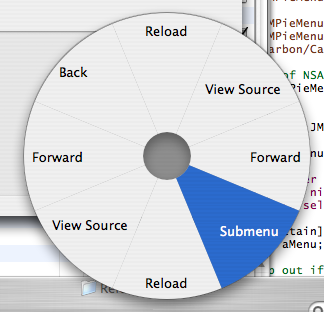
\includegraphics[scale=0.5]{30-10-15-01}
  \caption{Esempio di Pie Menu}
\end{figure}
